%!TEX root = ../main.tex
\chapter{Gravitazione}

\section{Le leggi di Keplero}

Dal punto di vista storico la gravitazione universale è frutto di osservazioni sperimentali di diversi fisici. Agli inizi del 1500 era stata avanzata da Copernico l'ipotesi eliocentrica: il Sole, e non la Terra, è il corpo celeste attorno al quale si svolge il moto dei pianeti. Successivamente, le posizioni assunte da questi ultimi nel tempo erano state oggetto di numerose e accurate misure da parte di Brahe alla fine del '500. Su tali misure si basò Keplero per formulare, tra il 1600 e il 1620, le sue tre leggi.

\textbf{Prima legge}

\noindent\fbox{%
	\parbox{\textwidth}{%
		\emph{I pianeti percorrono orbite ellittiche intorno al Sole che occupa uno dei fuochi dell'ellisse.}
	}%
}

In tale ambito, si definisce l'eccentricità di un'ellisse come il rapporto fra asse maggiore e asse minore. Se è uguale a uno è una circonferenza, se tende a infinito l'ellisse degenera in una retta (e il punto andrebbe avanti e indietro).

\textbf{Seconda legge} 

\noindent\fbox{%
	\parbox{\textwidth}{%
		\emph{La velocità areale con cui il raggio vettore che unisce il Sole ad un pianeta descrive l'orbita è costante.}
	}%
}

Questa legge è formulata anche dicendo che il punto spazza aree uguali in tempi uguali. Si immagini che mentre il pianeta ruota il raggio vettore lasci una traccia, in un tempo $\Delta t$ avrà spaziato un area.

\begin{figure}[htpb]
	\centering

	% Pattern Info
	 
	\tikzset{
	pattern size/.store in=\mcSize, 
	pattern size = 5pt,
	pattern thickness/.store in=\mcThickness, 
	pattern thickness = 0.3pt,
	pattern radius/.store in=\mcRadius, 
	pattern radius = 1pt}
	\makeatletter
	\pgfutil@ifundefined{pgf@pattern@name@_wlc8yueuj}{
	\pgfdeclarepatternformonly[\mcThickness,\mcSize]{_wlc8yueuj}
	{\pgfqpoint{0pt}{-\mcThickness}}
	{\pgfpoint{\mcSize}{\mcSize}}
	{\pgfpoint{\mcSize}{\mcSize}}
	{
	\pgfsetcolor{\tikz@pattern@color}
	\pgfsetlinewidth{\mcThickness}
	\pgfpathmoveto{\pgfqpoint{0pt}{\mcSize}}
	\pgfpathlineto{\pgfpoint{\mcSize+\mcThickness}{-\mcThickness}}
	\pgfusepath{stroke}
	}}
	\makeatother

	% Pattern Info
	 
	\tikzset{
	pattern size/.store in=\mcSize, 
	pattern size = 5pt,
	pattern thickness/.store in=\mcThickness, 
	pattern thickness = 0.3pt,
	pattern radius/.store in=\mcRadius, 
	pattern radius = 1pt}
	\makeatletter
	\pgfutil@ifundefined{pgf@pattern@name@_vq8azi3lx}{
	\pgfdeclarepatternformonly[\mcThickness,\mcSize]{_vq8azi3lx}
	{\pgfqpoint{0pt}{-\mcThickness}}
	{\pgfpoint{\mcSize}{\mcSize}}
	{\pgfpoint{\mcSize}{\mcSize}}
	{
	\pgfsetcolor{\tikz@pattern@color}
	\pgfsetlinewidth{\mcThickness}
	\pgfpathmoveto{\pgfqpoint{0pt}{\mcSize}}
	\pgfpathlineto{\pgfpoint{\mcSize+\mcThickness}{-\mcThickness}}
	\pgfusepath{stroke}
	}}
	\makeatother
	\tikzset{every picture/.style={line width=0.75pt}} %set default line width to 0.75pt        

	\begin{tikzpicture}[x=0.75pt,y=0.75pt,yscale=-1,xscale=1]
	%uncomment if require: \path (0,300); %set diagram left start at 0, and has height of 300

	%Shape: Polygon Curved [id:ds7888048739385256] 
	\draw  [draw opacity=0][pattern=_wlc8yueuj,pattern size=3.75pt,pattern thickness=0.75pt,pattern radius=0pt, pattern color={rgb, 255:red, 222; green, 222; blue, 222}] (366.5,194) .. controls (354.5,182.75) and (344.5,173.75) .. (316.75,148) .. controls (340.5,124.75) and (349.5,116.75) .. (366.5,100) .. controls (385,140.75) and (381.5,162.25) .. (366.5,194) -- cycle ;
	%Shape: Polygon Curved [id:ds3660792116229794] 
	\draw  [draw opacity=0][pattern=_vq8azi3lx,pattern size=3.75pt,pattern thickness=0.75pt,pattern radius=0pt, pattern color={rgb, 255:red, 222; green, 222; blue, 222}] (122.5,121) .. controls (164,126.75) and (267.5,140.75) .. (316.75,148) .. controls (258,148.25) and (172,149.75) .. (118.5,151) .. controls (117.5,141.25) and (120,129.75) .. (122.5,121) -- cycle ;
	%Shape: Ellipse [id:dp10272028811620681] 
	\draw   (118,148) .. controls (118,88.35) and (176.54,40) .. (248.75,40) .. controls (320.96,40) and (379.5,88.35) .. (379.5,148) .. controls (379.5,207.65) and (320.96,256) .. (248.75,256) .. controls (176.54,256) and (118,207.65) .. (118,148) -- cycle ;
	%Straight Lines [id:da08228735118508945] 
	\draw    (366.5,100) -- (316.75,148) ;
	%Straight Lines [id:da8949547722445947] 
	\draw    (366.5,194) -- (316.75,148) ;
	%Straight Lines [id:da6396212065868376] 
	\draw    (316.75,148) -- (122.5,121) ;
	%Straight Lines [id:da132233877114581] 
	\draw    (316.75,148) -- (118.5,151) ;
	%Straight Lines [id:da14243283627350656] 
	\draw    (179.5,229.47) -- (316.75,148) ;
	\draw [shift={(176.92,231)}, rotate = 329.31] [fill={rgb, 255:red, 0; green, 0; blue, 0 }  ][line width=0.08]  [draw opacity=0] (10.72,-5.15) -- (0,0) -- (10.72,5.15) -- (7.12,0) -- cycle    ;
	%Shape: Circle [id:dp19722738347889135] 
	\draw  [draw opacity=0][fill={rgb, 255:red, 184; green, 184; blue, 184 }  ,fill opacity=1 ] (301,148) .. controls (301,139.3) and (308.05,132.25) .. (316.75,132.25) .. controls (325.45,132.25) and (332.5,139.3) .. (332.5,148) .. controls (332.5,156.7) and (325.45,163.75) .. (316.75,163.75) .. controls (308.05,163.75) and (301,156.7) .. (301,148) -- cycle ;
	%Shape: Circle [id:dp22507537647047027] 
	\draw  [draw opacity=0][fill={rgb, 255:red, 128; green, 128; blue, 128 }  ,fill opacity=1 ] (164.42,235) .. controls (164.42,231.09) and (167.59,227.92) .. (171.5,227.92) .. controls (175.41,227.92) and (178.58,231.09) .. (178.58,235) .. controls (178.58,238.91) and (175.41,242.08) .. (171.5,242.08) .. controls (167.59,242.08) and (164.42,238.91) .. (164.42,235) -- cycle ;

	% Text Node
	\draw (136,137) node    {$A_{1}$};
	% Text Node
	\draw (354,145) node    {$A_{2}$};
	% Text Node
	\draw (438.5,140.5) node    {$A_{1} =A_{2}$};
	% Text Node
	\draw (269.33,214.67) node   [align=left] {raggio vettore};
	% Text Node
	\draw (142.67,251.33) node   [align=left] {pianeta};
	% Text Node
	\draw (311.33,120) node   [align=left] {Sole};

	\end{tikzpicture}
\end{figure}
\FloatBarrier
Quando il pianeta è lontano dal Sole esso si muoverà più lentamente, viceversa la velocità sarà massima quando si troverà molto vicino ad esso. In un'ellisse i punti in cui l'asse maggiore interseca tale curva sono rispettivamente il punto di minima e massima distanza dal fuoco. Essi prendono il nome di \textbf{perielio} e \textbf{afelio}.

\textbf{Terza legge} 

\noindent\fbox{%
	\parbox{\textwidth}{%
		\emph{Detto $T$ il periodo impiegato da un pianeta per compiere un giro intorno al Sole (periodo di rivoluzione), si osserva che il quadrato del periodo di rivoluzione di ogni pianeta è proporzionale al cubo del semiasse maggiore.} \[T^2=kr^3\]
	}%
}

Questa proporzionalità è la stessa per tutti i pianeti del sistema solare. La costante non dipende dalla massa del pianeta che sta ruotando. Tale legge mette in evidenza un legame fra tutti i pianeti del sistema solare: quelli più lontani dal Sole orbiteranno con un tempo ovviamente più lungo per mantenere la proporzionalità.

\section{Forza di gravitazione universale}

Fu poi Newton a dare una interpretazione metodologica, basata su un concetto fisico, di queste tre osservazioni sperimentali attuate da Keplero. Se esse infatti danno una descrizione cinematica del moto dei pianeti, la spiegazione dinamica venne trovata proprio da Newton nel 1666. Affinché le tre leggi siano vere, il corpo non può che essere soggetto a un'unica forza detta di gravitazione universale. Essa è tale per cui, detta $r$ la mutua distanza fra i centri dei pianeti,  è inversamente proporzionale al quadrato di $r$ e direttamente proporzionale al prodotto fra le masse, tramite una costante di proporzionalità. Immaginando che la massa $M$ sia il Sole e la $m$ sia il pianeta, si ha:

\[
	\norm{\vec{F}_\gamma}=\frac{mM}{r^2}\gamma \qquad \text{con} \quad\gamma=6.67 \cdot 10^{-11} m^3 kg^{-1} s^{-2}
\]

Fu poi Cavendish a capire che doveva trattarsi di una forza attrattiva fra due corpi.

\begin{figure}[htpb]
	\centering

	\tikzset{every picture/.style={line width=0.75pt}} %set default line width to 0.75pt        

	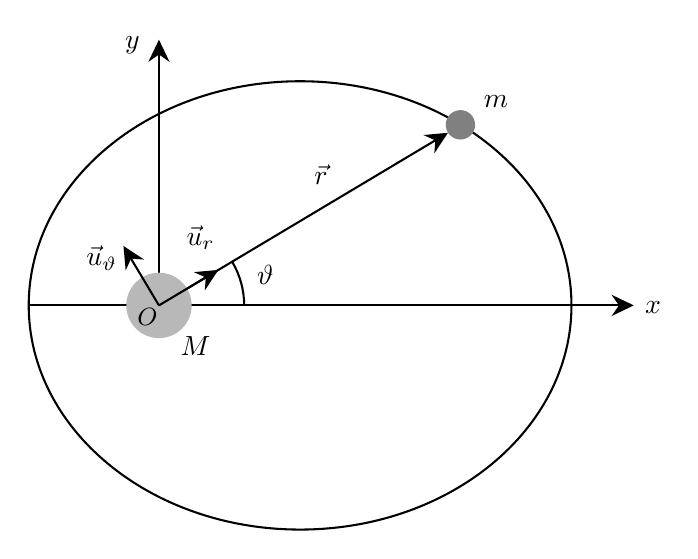
\begin{tikzpicture}[x=0.75pt,y=0.75pt,yscale=-1,xscale=1]
	%uncomment if require: \path (0,300); %set diagram left start at 0, and has height of 300

	%Shape: Ellipse [id:dp9941739679943589] 
	\draw   (399.5,168) .. controls (399.5,227.65) and (340.96,276) .. (268.75,276) .. controls (196.54,276) and (138,227.65) .. (138,168) .. controls (138,108.35) and (196.54,60) .. (268.75,60) .. controls (340.96,60) and (399.5,108.35) .. (399.5,168) -- cycle ;
	%Shape: Circle [id:dp0635364371860474] 
	\draw  [draw opacity=0][fill={rgb, 255:red, 128; green, 128; blue, 128 }  ,fill opacity=1 ] (353.08,81) .. controls (353.08,84.91) and (349.91,88.08) .. (346,88.08) .. controls (342.09,88.08) and (338.92,84.91) .. (338.92,81) .. controls (338.92,77.09) and (342.09,73.92) .. (346,73.92) .. controls (349.91,73.92) and (353.08,77.09) .. (353.08,81) -- cycle ;
	%Straight Lines [id:da5431299853077853] 
	\draw    (426.5,168) -- (138,168) ;
	\draw [shift={(429.5,168)}, rotate = 180] [fill={rgb, 255:red, 0; green, 0; blue, 0 }  ][line width=0.08]  [draw opacity=0] (10.72,-5.15) -- (0,0) -- (10.72,5.15) -- (7.12,0) -- cycle    ;
	%Straight Lines [id:da6109887920330987] 
	\draw    (200.75,43) -- (200.75,168) ;
	\draw [shift={(200.75,40)}, rotate = 90] [fill={rgb, 255:red, 0; green, 0; blue, 0 }  ][line width=0.08]  [draw opacity=0] (10.72,-5.15) -- (0,0) -- (10.72,5.15) -- (7.12,0) -- cycle    ;
	%Straight Lines [id:da08744928129546925] 
	\draw    (337.42,86.37) -- (200.75,168) ;
	\draw [shift={(340,84.83)}, rotate = 149.15] [fill={rgb, 255:red, 0; green, 0; blue, 0 }  ][line width=0.08]  [draw opacity=0] (10.72,-5.15) -- (0,0) -- (10.72,5.15) -- (7.12,0) -- cycle    ;
	%Shape: Arc [id:dp006379504475305886] 
	\draw  [draw opacity=0] (235.99,146.94) .. controls (239.68,153.1) and (241.8,160.3) .. (241.8,168) -- (200.75,168) -- cycle ; \draw   (235.99,146.94) .. controls (239.68,153.1) and (241.8,160.3) .. (241.8,168) ;
	%Shape: Circle [id:dp6764092735681855] 
	\draw  [draw opacity=0][fill={rgb, 255:red, 184; green, 184; blue, 184 }  ,fill opacity=1 ] (216.5,168) .. controls (216.5,176.7) and (209.45,183.75) .. (200.75,183.75) .. controls (192.05,183.75) and (185,176.7) .. (185,168) .. controls (185,159.3) and (192.05,152.25) .. (200.75,152.25) .. controls (209.45,152.25) and (216.5,159.3) .. (216.5,168) -- cycle ;
	%Shape: Boxed Line [id:dp8971684018104789] 
	\draw    (226.82,152.43) -- (200.75,168) ;
	\draw [shift={(229.4,150.89)}, rotate = 149.15] [fill={rgb, 255:red, 0; green, 0; blue, 0 }  ][line width=0.08]  [draw opacity=0] (10.72,-5.15) -- (0,0) -- (10.72,5.15) -- (7.12,0) -- cycle    ;
	%Shape: Boxed Line [id:dp9239139265790635] 
	\draw    (185.18,141.93) -- (200.75,168) ;
	\draw [shift={(183.64,139.35)}, rotate = 59.15] [fill={rgb, 255:red, 0; green, 0; blue, 0 }  ][line width=0.08]  [draw opacity=0] (10.72,-5.15) -- (0,0) -- (10.72,5.15) -- (7.12,0) -- cycle    ;

	% Text Node
	\draw (252,153.2) node    {$\vartheta $};
	% Text Node
	\draw (438.8,168.8) node    {$x$};
	% Text Node
	\draw (188,42.8) node    {$y$};
	% Text Node
	\draw (173.2,145.2) node    {$\vec{u}_{\vartheta }$};
	% Text Node
	\draw (220.8,135.2) node    {$\vec{u}_{r}$};
	% Text Node
	\draw (195.27,173.4) node  [font=\small]  {$O$};
	% Text Node
	\draw (218.4,187.6) node    {$M$};
	% Text Node
	\draw (363.2,69.6) node    {$m$};
	% Text Node
	\draw (278.8,105.2) node    {$\vec{r}$};

	\end{tikzpicture}
\end{figure}
\FloatBarrier
Invece che un sistema di riferimento cartesiano, in tale ambito risulta più pratico l'utilizzo di un sistema di riferimento in coordinate polari, dove il centro viene messo in corrispondenza del corpo attrattore. Si va poi a identificare il raggio vettore $\vec{r}$.  La posizione $P$ è identificata da una coppia di valori: la distanza radiale (lunghezza del raggio vettore) e l'angolo $\vartheta$, formato da $\vec{r}$ e da una direzione di riferimento fissa (ad esempio l'asse orizzontale). Ecco le relazioni che intercorrono con il sistema cartesiano:

\begin{gather*}
	\begin{cases} x=r\cos\vartheta \\ y=r\sin\vartheta \end{cases} \iff P(r,\vartheta)=P(x,y) \\
	r=\sqrt{x^2+y^2} \qquad \tan\vartheta=\frac{y}{x}
\end{gather*}

Si definiscono i versori $\vec{u}_r$ e $\vec{u}_\vartheta$, tangente alla traiettoria e con verso concorde a quello di percorrenza. A questo punto diventa molto semplice esprimere la forza gravitazionale in forma vettoriale.

\[
	\boxed{\vec{F}=-\frac{mM}{r^2}\gamma\, \vec{u}_r}
\]

Si noti che la forza di gravitazione universale è una \textbf{forza centrale}. In meccanica classica, una forza centrale è una forza diretta lungo la congiungente del punto di applicazione e un punto fisso, detto centro della forza, e tale che in ogni momento il modulo sia funzione esclusivamente del raggio-vettore tra il punto di applicazione della forza e il centro. Conseguenza di ciò è che la forza di interazione gravitazionale permette la conservazione del momento angolare ed è conservativa. Questi fatti verranno affrontati in seguito.

La velocità del punto materiale ha in generale una componente che è parallela al raggio, \emph{velocità radiale} e una ortogonale ad esso, \emph{velocità trasversa}. Durante il moto la velocità radiale dice quanto rapidamente il pianeta si avvicina o si allontana dal Sole. L'altra informa su quanto rapidamente esso sta ruotando intorno a questo.
Si ricava la loro espressione:

\begin{gather*}
	\vec{v}=\frac{d\vec{r}}{dt}=\frac{d(r\vec{u}_r)}{dt}=\frac{dr}{dt}\,\vec{u}_r+r\,\frac{d\vec{u}_r}{dt}=\frac{dr}{dt}\,\vec{u}_r+r\frac{d\vartheta}{dt}\,\vec{u}_\vartheta=\vec{v}_r+r\underbrace{(\vec{\omega}\times\vec{u}_r)}_{\text{vettore $\parallel$ a } \vec{u}_\vartheta} \\
	\vec{v}=\vec{v}_r+r\frac{d\vartheta}{dt}\, \vec{u}_\vartheta \implies \vec{v}=\vec{v}_r+\vec{v}_\vartheta
\end{gather*}

\begin{figure}[htpb]
	\centering

	\tikzset{every picture/.style={line width=0.75pt}} %set default line width to 0.75pt        

	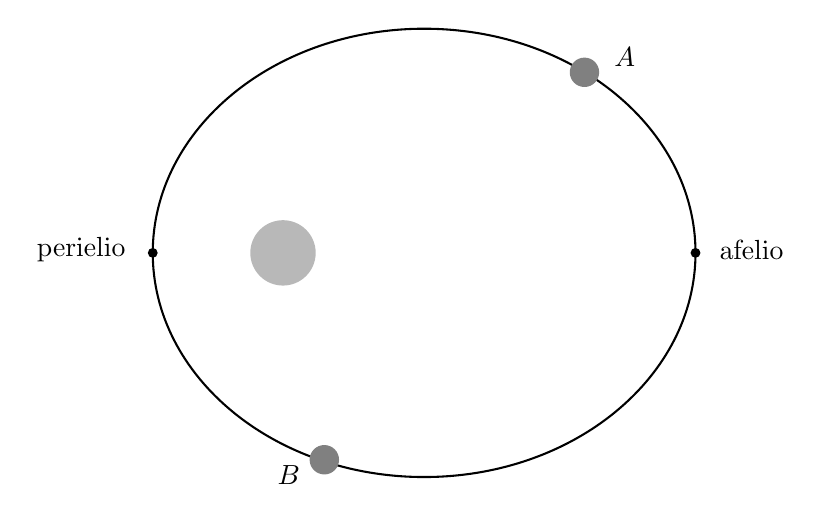
\begin{tikzpicture}[x=0.75pt,y=0.75pt,yscale=-1,xscale=1]
	%uncomment if require: \path (0,300); %set diagram left start at 0, and has height of 300

	%Shape: Ellipse [id:dp41169445171757313] 
	\draw   (394.5,169) .. controls (394.5,228.65) and (335.96,277) .. (263.75,277) .. controls (191.54,277) and (133,228.65) .. (133,169) .. controls (133,109.35) and (191.54,61) .. (263.75,61) .. controls (335.96,61) and (394.5,109.35) .. (394.5,169) -- cycle ;
	%Shape: Circle [id:dp19752370514212458] 
	\draw  [draw opacity=0][fill={rgb, 255:red, 128; green, 128; blue, 128 }  ,fill opacity=1 ] (348.08,82) .. controls (348.08,85.91) and (344.91,89.08) .. (341,89.08) .. controls (337.09,89.08) and (333.92,85.91) .. (333.92,82) .. controls (333.92,78.09) and (337.09,74.92) .. (341,74.92) .. controls (344.91,74.92) and (348.08,78.09) .. (348.08,82) -- cycle ;
	%Shape: Circle [id:dp9056973707211953] 
	\draw  [draw opacity=0][fill={rgb, 255:red, 184; green, 184; blue, 184 }  ,fill opacity=1 ] (211.5,169) .. controls (211.5,177.7) and (204.45,184.75) .. (195.75,184.75) .. controls (187.05,184.75) and (180,177.7) .. (180,169) .. controls (180,160.3) and (187.05,153.25) .. (195.75,153.25) .. controls (204.45,153.25) and (211.5,160.3) .. (211.5,169) -- cycle ;
	%Shape: Circle [id:dp03866659809345174] 
	\draw  [fill={rgb, 255:red, 0; green, 0; blue, 0 }  ,fill opacity=1 ] (131.17,169) .. controls (131.17,167.99) and (131.99,167.17) .. (133,167.17) .. controls (134.01,167.17) and (134.83,167.99) .. (134.83,169) .. controls (134.83,170.01) and (134.01,170.83) .. (133,170.83) .. controls (131.99,170.83) and (131.17,170.01) .. (131.17,169) -- cycle ;
	%Shape: Circle [id:dp785149968468944] 
	\draw  [fill={rgb, 255:red, 0; green, 0; blue, 0 }  ,fill opacity=1 ] (392.67,169) .. controls (392.67,167.99) and (393.49,167.17) .. (394.5,167.17) .. controls (395.51,167.17) and (396.33,167.99) .. (396.33,169) .. controls (396.33,170.01) and (395.51,170.83) .. (394.5,170.83) .. controls (393.49,170.83) and (392.67,170.01) .. (392.67,169) -- cycle ;
	%Shape: Circle [id:dp3881830809031668] 
	\draw  [draw opacity=0][fill={rgb, 255:red, 128; green, 128; blue, 128 }  ,fill opacity=1 ] (222.75,268.67) .. controls (222.75,272.58) and (219.58,275.75) .. (215.67,275.75) .. controls (211.75,275.75) and (208.58,272.58) .. (208.58,268.67) .. controls (208.58,264.75) and (211.75,261.58) .. (215.67,261.58) .. controls (219.58,261.58) and (222.75,264.75) .. (222.75,268.67) -- cycle ;

	% Text Node
	\draw (360.47,74.47) node    {$A$};
	% Text Node
	\draw (198.5,276.13) node    {$B$};
	% Text Node
	\draw (98.5,167.5) node   [align=left] {perielio};
	% Text Node
	\draw (421.5,167.5) node   [align=left] {afelio};

	\end{tikzpicture}
\end{figure}
\FloatBarrier
Si noti che in corrispondenza dell'afelio e del perielio la componente radiale non c'è, la velocità ha soltanto componente trasversale. Ciò accade perché la velocità radiale informa su come varia la distanza dal Sole. Essa diminuisce, raggiunge un punto di minimo, poi aumenta fino a raggiungere il massimo e via dicendo. $r(\vartheta)$ varia come in figura. Per i valori che corrispondono all'afelio e al perielio si hanno punti a tangente orizzontale. In corrispondenza di questi la derivata non può che essere nulla.

\begin{figure}[htpb]
	\centering

	\tikzset{every picture/.style={line width=0.75pt}} %set default line width to 0.75pt        

	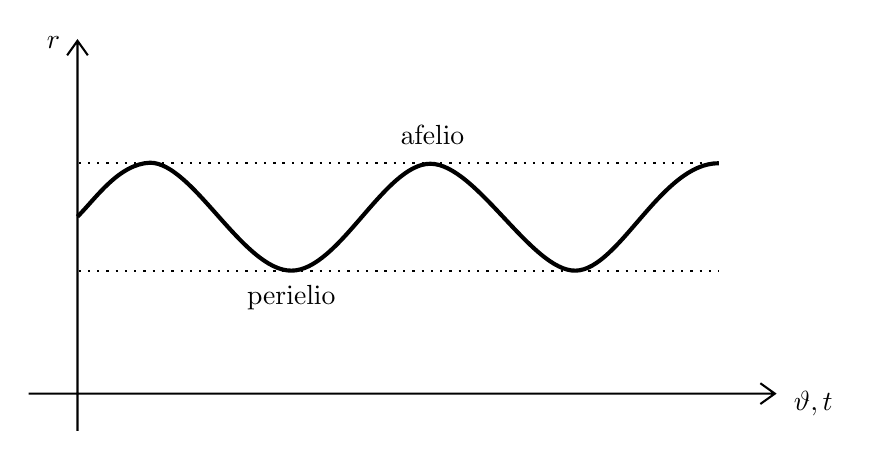
\begin{tikzpicture}[x=0.75pt,y=0.75pt,yscale=-1,xscale=1]
	%uncomment if require: \path (0,300); %set diagram left start at 0, and has height of 300

	% Plotting does not support converting to Tikz
	%Shape: Axis 2D [id:dp6077987803013458] 
	\draw  (81,241) -- (440.5,241)(104.5,71) -- (104.5,259) (433.5,236) -- (440.5,241) -- (433.5,246) (99.5,78) -- (104.5,71) -- (109.5,78)  ;
	%Straight Lines [id:da7365662394897443] 
	\draw  [dash pattern={on 0.84pt off 2.51pt}]  (105,130) -- (413.5,130) ;
	%Straight Lines [id:da7879993821891] 
	\draw  [dash pattern={on 0.84pt off 2.51pt}]  (105,182) -- (413.5,182) ;
	%Curve Lines [id:da7192072802610738] 
	\draw [line width=1.5]    (104.5,155.75) .. controls (113.5,146.75) and (124.5,130.25) .. (139.5,129.75) .. controls (160,129.75) and (184.5,181.75) .. (207.5,181.75) .. controls (230.5,181.75) and (252.5,130.25) .. (274.5,130.25) .. controls (296.5,130.25) and (323.5,182.25) .. (344.5,181.75) .. controls (365.5,181.25) and (386,129.75) .. (413.5,130) ;

	% Text Node
	\draw (207.5,194.5) node   [align=left] {perielio};
	% Text Node
	\draw (275.5,116.5) node   [align=left] {afelio};
	% Text Node
	\draw (93,72) node    {$r$};
	% Text Node
	\draw (459,246) node    {$\vartheta ,t$};

	\end{tikzpicture}
\end{figure}
\FloatBarrier
Si noti che la forza gravitazionale non è una forza centripeta. Per esserlo dovrebbe essere diretta perpendicolarmente alla traiettoria. Ma essa ha sia una componente tangente che una trasversale. Ci sono solo due punti in cui la forza gravitazionale si comporta come forza centripeta in un'orbita ellittica, e questi sono proprio l'afelio e il perielio. Si osserva però che, in generale:

\[
	\gamma\,\frac{mM}{r_\text{afelio}^2}=\frac{mv_\text{afelio}^2}{r_\text{afelio}}
\]

Si noti che, a differenza delle forze finora considerate, che si manifestano al contatto macroscopico tra i corpi, la forza gravitazionale si manifesta a distanza, senza che le masse vengono a contatto. In effetti tutte le interazioni fondamentali conosciute sono forze a distanza, che differiscono però nel raggio di azione (oltre che per altre proprietà): la forza gravitazionale e la forza tra cariche elettriche hanno la stessa dipendenza dalla distanza e si dice che il loro raggio di azione è infinito, invece la forza forte e quella debole decrescono molto più rapidamente con la distanza e sono efficaci solo a livello subatomico.

\section{Verifica delle leggi di Keplero}

La forza gravitazionale rispetto al polo non genera momento perché non ha una componente ortogonale al raggio vettore, ma è sempre parallela ad esso: come diretta conseguenza, un pianeta ha un momento angolare costante nel tempo. Esso non collassa perché è in movimento, la sua velocità iniziale gli permette di ruotare. L'obbiettivo è studiare quali sono gli effetti cinematici che ciò comporta. Verrebbe da pensare che il punto si muove di moto circolare uniforme, ma questo è solo un caso particolare della situazione che si presenta.
Si consideri un oggetto che si muove su una traiettoria con momento angolare costante, in direzione, verso e modulo.

\paragraph{1} La conseguenza del fatto che la direzione di $\vec{L}$ si mantiene costante è che il moto non può essere tridimensionale, ma avviene su un piano, formato da $\vec{r}$ e $\vec{v}$. Si ha così una verifica della prima legge di Keplero. Il verso di $\vec{L}$ costante vuol dire invece che il punto non può mai invertire il moto.

\paragraph{2} Si calcoli ora il modulo del momento angolare:

\[
	\norm{\vec{L}}=\norm{\vec{r}\times m\vec{v}}=\norm{\vec{r}\times m(\vec{v}_r+\vec{v}_\vartheta)}=\norm{\vec{r}\times m \vec{v}_\vartheta}
\]
$\vec{r}$ e $\vec{v}_\vartheta$ sono ortogonali quindi il prodotto vettoriale fra di essi non è altro che il prodotto fra i loro moduli.

\[
	\norm{\vec{L}}=\norm{\vec{r}} \cdot \norm{\vec{v}_\vartheta} m=r^2\omega m=m\,r^2\,\frac{d\vartheta}{dt}=\text{costante}
\]

Si immagini che il punto si stia muovendo di un piccolo tratto infinitesimo:  la sua posizione angolare varia di $d\vartheta$. Si definisce \textbf{velocità areale} o areoale, $\frac{dA}{dt}$, la quantità scalare pari alla variazione nel tempo dell'area spaziata dal raggio vettore. Si procede approssimando l'area tratteggiata all'area di un triangolo.

\begin{figure}[htpb]
	\centering

	% Pattern Info
	 
	\tikzset{
	pattern size/.store in=\mcSize, 
	pattern size = 5pt,
	pattern thickness/.store in=\mcThickness, 
	pattern thickness = 0.3pt,
	pattern radius/.store in=\mcRadius, 
	pattern radius = 1pt}
	\makeatletter
	\pgfutil@ifundefined{pgf@pattern@name@_ny7vciohh}{
	\pgfdeclarepatternformonly[\mcThickness,\mcSize]{_ny7vciohh}
	{\pgfqpoint{0pt}{-\mcThickness}}
	{\pgfpoint{\mcSize}{\mcSize}}
	{\pgfpoint{\mcSize}{\mcSize}}
	{
	\pgfsetcolor{\tikz@pattern@color}
	\pgfsetlinewidth{\mcThickness}
	\pgfpathmoveto{\pgfqpoint{0pt}{\mcSize}}
	\pgfpathlineto{\pgfpoint{\mcSize+\mcThickness}{-\mcThickness}}
	\pgfusepath{stroke}
	}}
	\makeatother
	\tikzset{every picture/.style={line width=0.75pt}} %set default line width to 0.75pt        

	\begin{tikzpicture}[x=0.75pt,y=0.75pt,yscale=-1,xscale=1]
	%uncomment if require: \path (0,300); %set diagram left start at 0, and has height of 300

	%Shape: Polygon Curved [id:ds16872019378222625] 
	\draw  [draw opacity=0][pattern=_ny7vciohh,pattern size=3pt,pattern thickness=0.75pt,pattern radius=0pt, pattern color={rgb, 255:red, 222; green, 222; blue, 222}] (249.2,65.4) .. controls (258.6,62.4) and (275,61.2) .. (283.75,61) .. controls (270.2,82.4) and (243,126.8) .. (215.75,169) .. controls (227,132.8) and (237.4,101.6) .. (249.2,65.4) -- cycle ;
	%Shape: Ellipse [id:dp9861585294009343] 
	\draw   (414.5,169) .. controls (414.5,228.65) and (355.96,277) .. (283.75,277) .. controls (211.54,277) and (153,228.65) .. (153,169) .. controls (153,109.35) and (211.54,61) .. (283.75,61) .. controls (355.96,61) and (414.5,109.35) .. (414.5,169) -- cycle ;
	%Straight Lines [id:da6105323859497809] 
	\draw    (215.75,169) -- (283.75,61) ;
	%Straight Lines [id:da870717036200692] 
	\draw    (215.75,169) -- (249.2,65.4) ;
	%Straight Lines [id:da7058693436437289] 
	\draw    (215.75,169) -- (264.72,64.91) ;
	\draw [shift={(266,62.2)}, rotate = 475.2] [fill={rgb, 255:red, 0; green, 0; blue, 0 }  ][line width=0.08]  [draw opacity=0] (10.72,-5.15) -- (0,0) -- (10.72,5.15) -- (7.12,0) -- cycle    ;
	%Shape: Circle [id:dp7452873351674358] 
	\draw  [draw opacity=0][fill={rgb, 255:red, 184; green, 184; blue, 184 }  ,fill opacity=1 ] (231.5,169) .. controls (231.5,177.7) and (224.45,184.75) .. (215.75,184.75) .. controls (207.05,184.75) and (200,177.7) .. (200,169) .. controls (200,160.3) and (207.05,153.25) .. (215.75,153.25) .. controls (224.45,153.25) and (231.5,160.3) .. (231.5,169) -- cycle ;
	%Straight Lines [id:da45722653487185494] 
	\draw    (250.18,57.02) -- (278.77,53.38) ;
	\draw [shift={(281.75,53)}, rotate = 532.74] [fill={rgb, 255:red, 0; green, 0; blue, 0 }  ][line width=0.08]  [draw opacity=0] (10.72,-5.15) -- (0,0) -- (10.72,5.15) -- (7.12,0) -- cycle    ;
	\draw [shift={(247.2,57.4)}, rotate = 352.74] [fill={rgb, 255:red, 0; green, 0; blue, 0 }  ][line width=0.08]  [draw opacity=0] (10.72,-5.15) -- (0,0) -- (10.72,5.15) -- (7.12,0) -- cycle    ;

	% Text Node
	\draw (263.77,37.77) node    {$rd\vartheta $};
	% Text Node
	\draw (260.27,116.47) node    {$\vec{r}$};

	\end{tikzpicture}
\end{figure}
\FloatBarrier
L'altezza è proprio la distanza radiale, la base $r\,d\vartheta$ è l'arco di circonferenza di raggio $r$ e ampiezza angolare $d\vartheta$.

\[
	v_\text{areale}=\frac{dA}{dt}=\frac{\frac{rd\vartheta\,r}{2}}{dt}=\frac{d\vartheta}{dt}\cdot \frac{1}{2} r^2=\frac{\omega r^2}{2}=\frac{v_\vartheta r}{2}=\frac{mv_\vartheta r}{2m}
\]

Quindi:

\[
	v_\text{areale}=\frac{\norm{\vec{L}}}{2m}
\]

Se il momento angolare è costante si ha che la velocità areale è costante. Trovare un moto in cui i momenti delle forze sono nulli e quindi il momento angolare è costante, vuole dire avere una traiettoria piana con velocità areale costante. Viene così verificata la seconda legge di Keplero.

\paragraph{Osservazione} È stato detto che il moto circolare uniforme è un caso particolare che si ha nel caso in cui il momento angolare è costante. Un corpo soggetto a forza gravitazionale che si muove lungo una traiettoria circolare mantiene costante la distanza con il pianeta attrattore. Il fatto che $\vec{r}$ sia costante implica l'assenza della componente radiale della velocità; in tutti i punti c'è solo la velocità trasversale. Infatti la velocità radiale dice quanto varia la distanza dal centro nel tempo, ma questa non cambia. È come se tutti i punti fossero l'afelio e il perielio.

\[
	v_\text{areale}=\frac{v_\vartheta r}{2}=\frac{\omega r^2}{2}
\]

Da questa espressione si vede che $r$ costante e velocità areale costante implicano una velocità angolare costante e quindi un moto uniforme.

\begin{figure}[htpb]
	\centering

	\tikzset{every picture/.style={line width=0.75pt}} %set default line width to 0.75pt        

	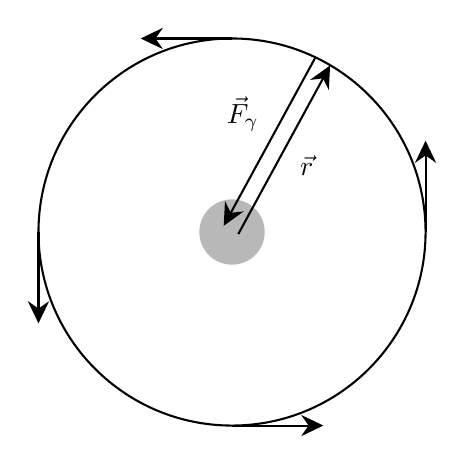
\begin{tikzpicture}[x=0.75pt,y=0.75pt,yscale=-1,xscale=1]
	%uncomment if require: \path (0,300); %set diagram left start at 0, and has height of 300

	%Straight Lines [id:da0745484543757402] 
	\draw    (444.5,162.25) -- (444.5,121.25) ;
	\draw [shift={(444.5,118.25)}, rotate = 450] [fill={rgb, 255:red, 0; green, 0; blue, 0 }  ][line width=0.08]  [draw opacity=0] (10.72,-5.15) -- (0,0) -- (10.72,5.15) -- (7.12,0) -- cycle    ;
	%Shape: Circle [id:dp6339082486573857] 
	\draw  [draw opacity=0][fill={rgb, 255:red, 184; green, 184; blue, 184 }  ,fill opacity=1 ] (367,162.25) .. controls (367,170.95) and (359.95,178) .. (351.25,178) .. controls (342.55,178) and (335.5,170.95) .. (335.5,162.25) .. controls (335.5,153.55) and (342.55,146.5) .. (351.25,146.5) .. controls (359.95,146.5) and (367,153.55) .. (367,162.25) -- cycle ;
	%Shape: Circle [id:dp6563003174772981] 
	\draw   (258,162.25) .. controls (258,110.75) and (299.75,69) .. (351.25,69) .. controls (402.75,69) and (444.5,110.75) .. (444.5,162.25) .. controls (444.5,213.75) and (402.75,255.5) .. (351.25,255.5) .. controls (299.75,255.5) and (258,213.75) .. (258,162.25) -- cycle ;
	%Straight Lines [id:da1874688148167316] 
	\draw    (258,203.25) -- (258,162.25) ;
	\draw [shift={(258,206.25)}, rotate = 270] [fill={rgb, 255:red, 0; green, 0; blue, 0 }  ][line width=0.08]  [draw opacity=0] (10.72,-5.15) -- (0,0) -- (10.72,5.15) -- (7.12,0) -- cycle    ;
	%Straight Lines [id:da038252941880675184] 
	\draw    (351.25,69) -- (310.25,69) ;
	\draw [shift={(307.25,69)}, rotate = 360] [fill={rgb, 255:red, 0; green, 0; blue, 0 }  ][line width=0.08]  [draw opacity=0] (10.72,-5.15) -- (0,0) -- (10.72,5.15) -- (7.12,0) -- cycle    ;
	%Straight Lines [id:da6941678012243162] 
	\draw    (392.25,255.5) -- (351.25,255.5) ;
	\draw [shift={(395.25,255.5)}, rotate = 180] [fill={rgb, 255:red, 0; green, 0; blue, 0 }  ][line width=0.08]  [draw opacity=0] (10.72,-5.15) -- (0,0) -- (10.72,5.15) -- (7.12,0) -- cycle    ;
	%Straight Lines [id:da6984646792309464] 
	\draw    (354.25,163.25) -- (397.07,84.63) ;
	\draw [shift={(398.5,82)}, rotate = 478.57] [fill={rgb, 255:red, 0; green, 0; blue, 0 }  ][line width=0.08]  [draw opacity=0] (10.72,-5.15) -- (0,0) -- (10.72,5.15) -- (7.12,0) -- cycle    ;
	%Straight Lines [id:da33278676717158584] 
	\draw    (348.68,156.62) -- (391.5,78) ;
	\draw [shift={(347.25,159.25)}, rotate = 298.57] [fill={rgb, 255:red, 0; green, 0; blue, 0 }  ][line width=0.08]  [draw opacity=0] (10.72,-5.15) -- (0,0) -- (10.72,5.15) -- (7.12,0) -- cycle    ;

	% Text Node
	\draw (387.27,130.47) node    {$\vec{r}$};
	% Text Node
	\draw (356.47,105.27) node    {$\vec{F}_{\gamma }$};

	\end{tikzpicture}
\end{figure}
\FloatBarrier
In questo particolare caso si ha:

\[
	\norm{\vec{F}_\gamma}=\gamma \frac{mM}{r^2}=m\omega^2r
\]

\paragraph{3} La terza legge di Keplero si dimostra qui nel caso di orbite circolari. Le orbite dei pianeti, pur essendo certamente ellittiche, sono molto prossime a circonferenze. Se la velocità areale è costante, il moto di un pianeta è circolare uniforme. Il periodo di rivoluzione, ossia il tempo per compiere un giro completo, è dato da:

\[
	T=\frac{2\pi}{\omega}
\]

La forza che agisce sul pianeta, permettendogli di percorrere una traiettoria circolare con velocità costante, deve essere esclusivamente centripeta, e si scrive:

\begin{gather*}
	F_\gamma=m\omega^2r \implies \omega^2=\frac{F_\gamma}{mr} \\
	T^2=\frac{4\pi^2}{\omega^2}=\frac{4\pi^2mr}{F_\gamma}=\frac{4\pi^2mr^3}{\gamma mM} \implies T^2=\underbrace{\frac{4\pi^2}{\gamma M}}_{=k} r^3 \implies T^2=kr^3
\end{gather*}

Questa relazione vale per tutti i pianeti del sistema solare perché non dipende dalla loro massa, ma solo da quella del pianeta attrattore, il Sole.

\section{Energia potenziale gravitazionale}

L'obbiettivo della sezione è quello di verificare se la forza gravitazionale è conservativa o meno.

\[
	\mathcal{L}=\int_{\Gamma, A\to B}\vec{F}_\gamma \cdot d\vec{r}
\]

\begin{figure}[htpb]
	\centering

	\tikzset{every picture/.style={line width=0.75pt}} %set default line width to 0.75pt        

	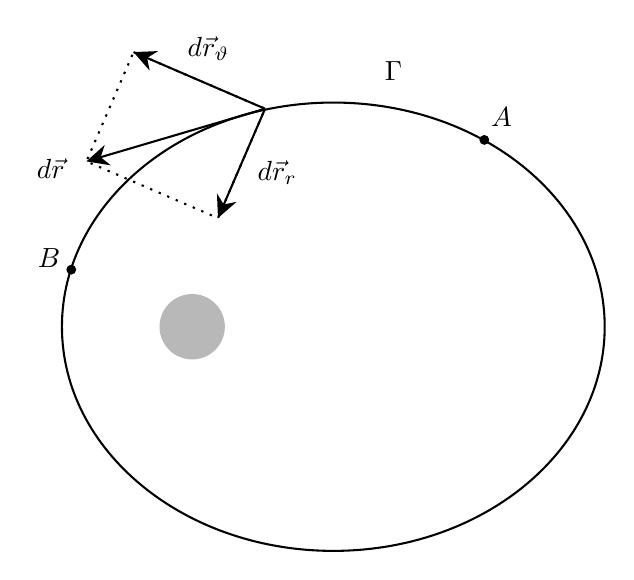
\begin{tikzpicture}[x=0.75pt,y=0.75pt,yscale=-1,xscale=1]
	%uncomment if require: \path (0,300); %set diagram left start at 0, and has height of 300

	%Shape: Ellipse [id:dp26398419772349535] 
	\draw   (434.5,189) .. controls (434.5,248.65) and (375.96,297) .. (303.75,297) .. controls (231.54,297) and (173,248.65) .. (173,189) .. controls (173,129.35) and (231.54,81) .. (303.75,81) .. controls (375.96,81) and (434.5,129.35) .. (434.5,189) -- cycle ;
	%Straight Lines [id:da6748300763011188] 
	\draw    (187.68,108.49) -- (270.86,83.99) ;
	\draw [shift={(184.81,109.34)}, rotate = 343.59] [fill={rgb, 255:red, 0; green, 0; blue, 0 }  ][line width=0.08]  [draw opacity=0] (10.72,-5.15) -- (0,0) -- (10.72,5.15) -- (7.12,0) -- cycle    ;
	%Shape: Rectangle [id:dp11471698125766983] 
	\draw  [dash pattern={on 0.84pt off 2.51pt}] (207.49,56.69) -- (270.86,83.99) -- (248.17,136.65) -- (184.81,109.34) -- cycle ;
	%Straight Lines [id:da37709233960590205] 
	\draw    (249.36,133.89) -- (270.86,83.99) ;
	\draw [shift={(248.17,136.65)}, rotate = 293.31] [fill={rgb, 255:red, 0; green, 0; blue, 0 }  ][line width=0.08]  [draw opacity=0] (10.72,-5.15) -- (0,0) -- (10.72,5.15) -- (7.12,0) -- cycle    ;
	%Straight Lines [id:da8201337662239865] 
	\draw    (210.25,57.88) -- (270.86,83.99) ;
	\draw [shift={(207.49,56.69)}, rotate = 23.31] [fill={rgb, 255:red, 0; green, 0; blue, 0 }  ][line width=0.08]  [draw opacity=0] (10.72,-5.15) -- (0,0) -- (10.72,5.15) -- (7.12,0) -- cycle    ;

	%Shape: Circle [id:dp4076016936839617] 
	\draw  [draw opacity=0][fill={rgb, 255:red, 184; green, 184; blue, 184 }  ,fill opacity=1 ] (251.5,189) .. controls (251.5,197.7) and (244.45,204.75) .. (235.75,204.75) .. controls (227.05,204.75) and (220,197.7) .. (220,189) .. controls (220,180.3) and (227.05,173.25) .. (235.75,173.25) .. controls (244.45,173.25) and (251.5,180.3) .. (251.5,189) -- cycle ;
	%Shape: Circle [id:dp7855035876590197] 
	\draw  [fill={rgb, 255:red, 0; green, 0; blue, 0 }  ,fill opacity=1 ] (175.67,161.5) .. controls (175.67,160.49) and (176.49,159.67) .. (177.5,159.67) .. controls (178.51,159.67) and (179.33,160.49) .. (179.33,161.5) .. controls (179.33,162.51) and (178.51,163.33) .. (177.5,163.33) .. controls (176.49,163.33) and (175.67,162.51) .. (175.67,161.5) -- cycle ;
	%Shape: Circle [id:dp9700834372146263] 
	\draw  [fill={rgb, 255:red, 0; green, 0; blue, 0 }  ,fill opacity=1 ] (374.67,99) .. controls (374.67,97.99) and (375.49,97.17) .. (376.5,97.17) .. controls (377.51,97.17) and (378.33,97.99) .. (378.33,99) .. controls (378.33,100.01) and (377.51,100.83) .. (376.5,100.83) .. controls (375.49,100.83) and (374.67,100.01) .. (374.67,99) -- cycle ;

	% Text Node
	\draw (384.77,87.77) node    {$A$};
	% Text Node
	\draw (167.6,112.63) node    {$d\vec{r}$};
	% Text Node
	\draw (166.77,155.77) node    {$B$};
	% Text Node
	\draw (243.6,55.13) node    {$d\vec{r}_{\vartheta }$};
	% Text Node
	\draw (276.77,114.8) node    {$d\vec{r}_{r}$};
	% Text Node
	\draw (332.77,65.77) node    {$\Gamma $};

	\end{tikzpicture}
\end{figure}
\FloatBarrier
Dove $d\vec{r}$ è il vettore spostamento, che non va confuso con il raggio. Lo si scompone in: $d\vec{r}=d\vec{r}_r+d\vec{r}_\vartheta$
A questo punto si ha:

\begin{align*}
	\mathcal{L} &= \int_{\Gamma, A \to B} \vec{F}_\gamma \cdot (d\vec{r}_r+d\vec{r}_\vartheta)=\int_{\Gamma, A \to B} \vec{F}_\gamma \cdot d\vec{r}_r= \int_{\Gamma, A \to B} -\gamma \frac{mM}{r^2}\,\vec{u}_r \cdot d\vec{r}_r= \\
	&= \int_{\Gamma, A \to B} - \gamma \frac{mM}{r^2} \,dr_r=-\gamma mM\,\biggl[-\frac{1}{r}\biggr]_{r_A}^{r_B}=\frac{\gamma mM}{r_B}-\frac{\gamma mM}{r_A}
\end{align*}

Contano soltanto la distanza radiale iniziale e quella finale, quindi la forza gravitazionale è conservativa. Si può definire la funzione energia potenziale imponendo che il lavoro sia pari all'opposto della sua variazione.

\[
	\boxed{E_{p,\text{gravitazionale}}=-\gamma \frac{mM}{r}+\text{cost}}
\]

Il pianeta orbitante tende ad essere portato verso il Sole, il segno negativo deriva dunque dal fatto che la forza gravitazionale è attrattiva. Se si sostituisce $r=0$, si ottiene energia potenziale infinita. È invece ragionevole che a distanza infinita, quindi quando non c'è interazione, l'energia potenziale sia nulla e quindi la costante si assume pari a $0$.

\begin{figure}[htpb]
	\centering

	\tikzset{every picture/.style={line width=0.75pt}} %set default line width to 0.75pt        

	\begin{tikzpicture}[x=0.75pt,y=0.75pt,yscale=-1,xscale=1]
	%uncomment if require: \path (0,325); %set diagram left start at 0, and has height of 325

	% Plotting does not support converting to Tikz
	%Shape: Axis 2D [id:dp4497706014371563] 
	\draw  (97,104) -- (435.5,104)(123.31,74) -- (123.31,286) (428.5,99) -- (435.5,104) -- (428.5,109) (118.31,81) -- (123.31,74) -- (128.31,81)  ;
	%Curve Lines [id:da8498389368782535] 
	\draw [line width=1.5]    (137,266) .. controls (141,100) and (230,125) .. (384,114) ;

	% Text Node
	\draw (105,70) node    {$E_{p}$};
	% Text Node
	\draw (452,102) node    {$r$};

	\end{tikzpicture}
\end{figure}
\FloatBarrier
Nell'applicare la definizione di lavoro se ne è andata la componente trasversale ed è rimasta quella radiale. Quella appena ricavata prendere il nome di \textbf{energia potenziale gravitazionale}.

Siccome la forza è conservativa, l'energia meccanica, somma dell'energia cinetica e dell'energia gravitazionale, resta costante e quindi se $E_k$ aumenta $E_p$ deve diminuire. Essendo nulla per distanza infinita, $E_p$ deve essere negativa per distante finite.

\[
	E_\text{mecc}=E_k+E_p=\frac{1}{2}mv^2-\gamma\frac{mM}{r}
\]

Riscrivendo l'energia cinetica nelle sue componenti radiale e trasversale:

\[
	E_\text{mecc}=\frac{1}{2}mv_r^2+\frac{1}{2}mv_\vartheta^2-\gamma \frac{mM}{r}=\frac{1}{2}mv_r^2+\underbrace{\underbrace{\frac{1}{2}\frac{\norm{\vec{L}}^2}{mr^2}}_B-\gamma\frac{mM}{r}}_A
\]

Per come è stato riscritto il termine $B$, esso è diventato una funzione che dipende da $L$, costante, e da un termine funzione della posizione. È allora un'energia posizionale, ossia potenziale. $A$ prende il nome di \textbf{energia potenziale gravitazionale efficace}. Si è attribuito così un significato fisico energetico diverso al secondo membro. Questa energia porta con sé una parte dell'energia cinetica, ma, in presenza di forze centrali, si può esprimere come funzione delle coordinate in quanto dipende solo dalla distanza di $m$ da $M$.

\section{Studio delle orbite}

In questa nuova visione si attribuisce al punto materiale un'unica energia cinetica che informa di quanto velocemente esso si allontana o si avvicina al Sole. È come se non si stesse più osservando il moto come osservatore assoluto posto in $O$, ma dal punto di vista di un osservatore relativo $O'$ che gira con la stessa velocità angolare del pianeta. $O'$ non lo vede muoversi, ma solo avvicinarsi e allontanarsi. Ponendosi come osservatore relativo, deve apparire una forza apparente centrifuga, opposta al raggio, che spiega lo spostamento del pianeta che $O'$ rileva. Essa nel sistema di riferimento apparente compie un lavoro pari al termine $B$. Si è così trasformato il problema dello studio del moto in un problema a una sola variabile, misurata rispetto alla coordinata radiale. L'energia potenziale efficace ha la forma rappresentata di seguito.

\begin{figure}[htpb]
	\centering

	\tikzset{every picture/.style={line width=0.75pt}} %set default line width to 0.75pt        

	\begin{tikzpicture}[x=0.75pt,y=0.75pt,yscale=-1,xscale=1]
	%uncomment if require: \path (0,346); %set diagram left start at 0, and has height of 346

	%Shape: Axis 2D [id:dp40528865472744124] 
	\draw  (117,185) -- (455.5,185)(142.5,78) -- (142.5,290) (448.5,180) -- (455.5,185) -- (448.5,190) (137.5,85) -- (142.5,78) -- (147.5,85)  ;
	%Curve Lines [id:da10823584761686678] 
	\draw [line width=1.5]    (142.5,97) .. controls (167,202.5) and (183,275.5) .. (233,276.5) .. controls (283,277.5) and (334,193.5) .. (399.5,194) ;

	% Text Node
	\draw (103,79) node    {$E_{p,\text{efficace}}$};
	% Text Node
	\draw (475,184) node    {$r$};

	\end{tikzpicture}
\end{figure}
\FloatBarrier
Per $r$ grande predomina il termine di energia potenziale gravitazionale. Quindi per $r$ che va a infinito il grafico approssima quello di $E_p$. Per $r$ che va a zero prevale l'energia potenziale efficace (centrifuga). In mezzo i due contributi pesano entrambi e danno luogo a un minimo relativo. L'energia cinetica radiale non può avere segno qualunque ma è sempre positiva o al massimo nulla. Questo vuole dire che la differenza fra l'energia totale e quella efficace gravitazionale deve essere sempre positiva.

\begin{gather*}
	E_\text{mecc}=E_\text{pot, eff}+E_\text{k, rad} \\
	E_\text{k,rad}=E_\text{mecc}-E_\text{pot, eff} >0 \implies E_\text{mecc}>E_\text{pot, eff}
\end{gather*}

Questa informazione è importante perché afferma che per il pianeta sono permesse solo quelle posizioni che fanno si che il grafico della sua energia meccanica sia sempre sopra al grafico dell'energia potenziale gravitazionale efficace. Se l'energia meccanica è al di sotto della curva, il pianeta non riesce a ruotare attorno al pianeta attrattore e collassa su di esso. Quelli sotto la curva sono valori di energia non permessi. L'energia totale può assumere valori positivi, negativi, o nulli.

Quando essa è positiva o nulla, $r$ ha un valore minimo. La distanza fra $M$ e $m$ non può scendere al di sotto di un certo valore che dipende da $E_\text{mecc}$ e da $L$. A parità di $E_\text{mecc}$, maggiore è $L$ maggiore è la distanza minima. Si osservi che quando $r$ è minimo, uno dei termini che compongono l'energia cinetica si annulla, per cui l'energia meccanica coincide con quella potenziale efficace.

\paragraph{1} Per $E_\text{mecc}=0$ le distanze consentite sono tutte quelle in cui l'energia meccanica sta sopra l'energia potenziale efficace. $r$ tenderà a infinito, nel punto di minimo la velocità ha soltanto componente trasversale e il punto si allontanerà all'infinito, facendo tendere l'energia potenziale efficace a $0$. La traiettoria è quella di una \textbf{parabola}. Anche l'energia cinetica radiale va a $0$. Quindi il punto arriva all'infinito con velocità nulla.

\paragraph{2} Per $E_\text{mecc}$ positiva si ha di nuovo una traiettoria aperta. Il pianeta arriva a distanza infinita avendo ancora energia cinetica radiale e quindi una certa velocità. Si può dimostrare che la traiettoria è un'\textbf{iperbole}.

\paragraph{3} Quando l'energia totale è negativa, la distanza fra $m$ e $M$ ha un valore minimo e massimo. Si può dimostrare che la traiettoria è appunto una \textbf{traiettoria ellittica} dove la distanza minima è il perielio e la massima è l'afelio. Nei punti $A$ e $B$ l'energia cinetica radiale è zero. In particolare, nel caso in cui l'energia meccanica ha valore pari a quello minimo dell'energia potenziale efficace, è permesso solo un valore di $r$ e quindi la configurazione è quella di un'\textbf{orbita circolare}, tutte le altre hanno un livello energetico superiore.

\begin{figure}[ht]
	\centering

	\tikzset{every picture/.style={line width=0.75pt}} %set default line width to 0.75pt        

	\begin{tikzpicture}[x=0.75pt,y=0.75pt,yscale=-1,xscale=1]
	%uncomment if require: \path (0,306); %set diagram left start at 0, and has height of 306

	%Shape: Axis 2D [id:dp06633050074921831] 
	\draw  (137,185) -- (475.5,185)(162.5,78) -- (162.5,290) (468.5,180) -- (475.5,185) -- (468.5,190) (157.5,85) -- (162.5,78) -- (167.5,85)  ;
	%Straight Lines [id:da8964693514751385] 
	\draw  [dash pattern={on 0.84pt off 2.51pt}]  (171.67,141.67) -- (171.67,185.67) ;
	%Straight Lines [id:da567489127467361] 
	\draw  [dash pattern={on 0.84pt off 2.51pt}]  (162.67,141.67) -- (394,141.67) ;
	%Curve Lines [id:da05339900489855598] 
	\draw [line width=1.5]    (162.5,100) .. controls (187,205.5) and (203,278.5) .. (253,279.5) .. controls (303,280.5) and (354,196.5) .. (419.5,197) ;

	% Text Node
	\draw (143,82) node    {$E_{p}$};
	% Text Node
	\draw (495,184) node    {$r$};
	% Text Node
	\draw (189.67,124.67) node    {$r_{min}$};
	% Text Node
	\draw (99,140) node    {$E_{\text{meccanica}} \geqslant 0$};

	\end{tikzpicture}
\end{figure}
\FloatBarrier

\begin{figure}[htpb]
	\centering

	\tikzset{every picture/.style={line width=0.75pt}} %set default line width to 0.75pt        

	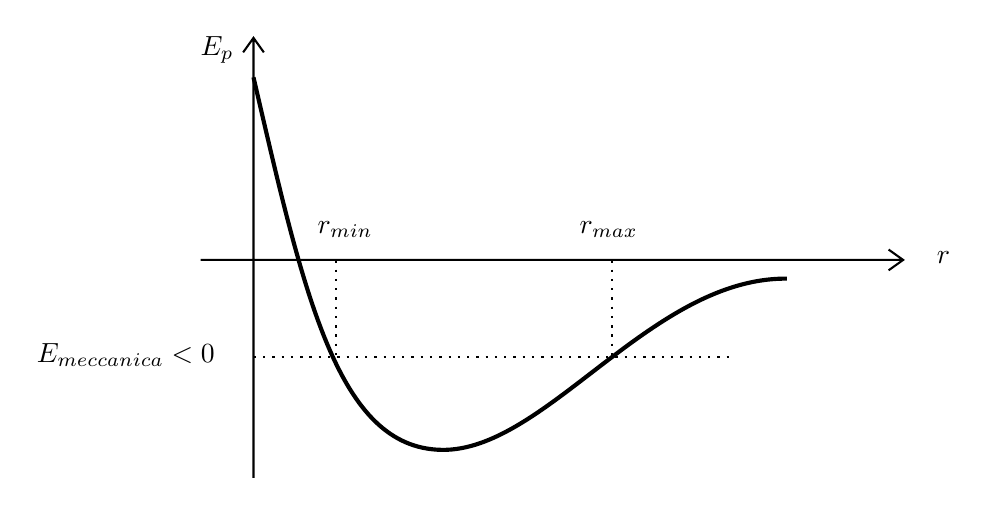
\begin{tikzpicture}[x=0.75pt,y=0.75pt,yscale=-1,xscale=1]
	%uncomment if require: \path (0,310); %set diagram left start at 0, and has height of 310

	%Shape: Axis 2D [id:dp6630535401419646] 
	\draw  (137,145) -- (475.5,145)(162.5,38) -- (162.5,250) (468.5,140) -- (475.5,145) -- (468.5,150) (157.5,45) -- (162.5,38) -- (167.5,45)  ;
	%Straight Lines [id:da10628897100542933] 
	\draw  [dash pattern={on 0.84pt off 2.51pt}]  (202.17,145.17) -- (202.17,191.17) ;
	%Straight Lines [id:da6958420279748636] 
	\draw  [dash pattern={on 0.84pt off 2.51pt}]  (162.67,191.67) -- (394,191.67) ;
	%Straight Lines [id:da07604953384880853] 
	\draw  [dash pattern={on 0.84pt off 2.51pt}]  (335.17,145.17) -- (335.17,191.17) ;
	%Curve Lines [id:da9957461492216604] 
	\draw [line width=1.5]    (162.5,57) .. controls (187,162.5) and (203,235.5) .. (253,236.5) .. controls (303,237.5) and (354,153.5) .. (419.5,154) ;

	% Text Node
	\draw (145,44) node    {$E_{p}$};
	% Text Node
	\draw (495,144) node    {$r$};
	% Text Node
	\draw (206.67,130.17) node    {$r_{min}$};
	% Text Node
	\draw (101,191) node    {$E_{\text{meccanica}} < 0$};
	% Text Node
	\draw (333.67,130.17) node    {$r_{max}$};

	\end{tikzpicture}
\end{figure}
\FloatBarrier
Quindi studiando il segno e il valore dell'energia totale si possono ottenere informazioni molto utili sulla forma della traiettoria seguita dal corpo. Si immagini ora di voler far partire un razzo dalla Terra. L'energia potenziale gravitazionale è fissata perché è nota la posizione del razzo. Perché esso possa decollare, gli si conferisce una certo valore della velocità, e quindi un'energia cinetica iniziale.
Dato che l'energia totale è costante, la somma di energia cinetica e potenziale dà un valore che a questo punto è fissato e che durante il moto si manterrà tale e quale. A seconda quindi della velocità che si conferisce al razzo, l'orbita percorsa sarà diversa e ci si riconduce a uno dei tre casi descritti in precedenza.

Oltre che scegliendo il modulo della velocità iniziale, si può far variare l'orbita seguita anche imponendo la direzione della velocità. Questo infatti si traduce nello stabilire un certo modulo del momento angolare. L'energia potenziale efficace dipende da quest'ultimo e quindi, nonostante mantenga la stessa forma, a seconda del valore di $L$ il suo andamento può allargarsi o restringersi.

\begin{figure}[htpb]
	\centering

	\tikzset{every picture/.style={line width=0.75pt}} %set default line width to 0.75pt        

	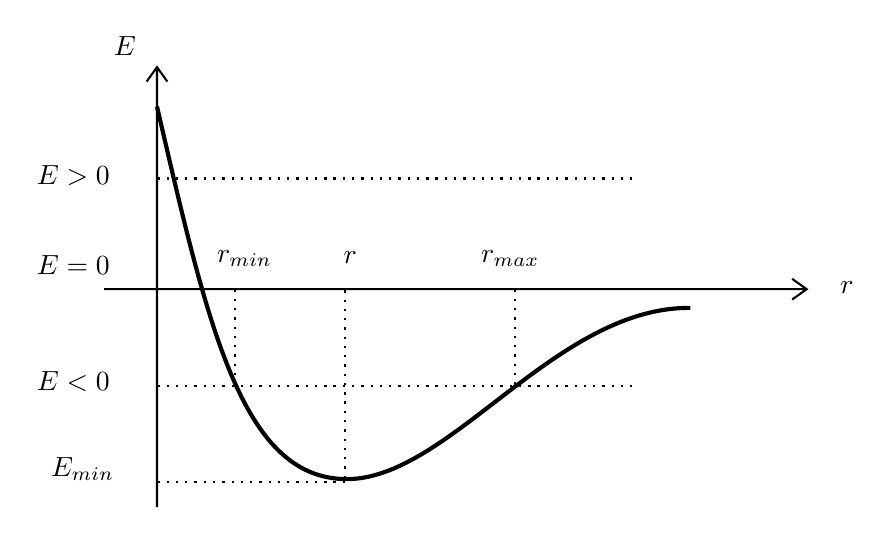
\begin{tikzpicture}[x=0.75pt,y=0.75pt,yscale=-1,xscale=1]
	%uncomment if require: \path (0,300); %set diagram left start at 0, and has height of 300

	%Shape: Axis 2D [id:dp008375906793796739] 
	\draw  (101,171) -- (439.5,171)(126.5,64) -- (126.5,276) (432.5,166) -- (439.5,171) -- (432.5,176) (121.5,71) -- (126.5,64) -- (131.5,71)  ;
	%Straight Lines [id:da17443468183766164] 
	\draw  [dash pattern={on 0.84pt off 2.51pt}]  (164.17,171.17) -- (164.17,217.17) ;
	%Straight Lines [id:da42800203214304755] 
	\draw  [dash pattern={on 0.84pt off 2.51pt}]  (126.67,217.67) -- (358,217.67) ;
	%Straight Lines [id:da9495313997069219] 
	\draw  [dash pattern={on 0.84pt off 2.51pt}]  (299.17,171.17) -- (299.17,217.17) ;
	%Straight Lines [id:da7012721870034195] 
	\draw  [dash pattern={on 0.84pt off 2.51pt}]  (126.67,117.67) -- (358,117.67) ;
	%Straight Lines [id:da7410405305183971] 
	\draw  [dash pattern={on 0.84pt off 2.51pt}]  (217.17,171.5) -- (217.17,263.17) ;
	%Straight Lines [id:da36685552188825965] 
	\draw  [dash pattern={on 0.84pt off 2.51pt}]  (126.67,263.67) -- (217,263.67) ;
	%Curve Lines [id:da2586176186680875] 
	\draw [line width=1.5]    (126.5,83) .. controls (151,188.5) and (167,261.5) .. (217,262.5) .. controls (267,263.5) and (318,179.5) .. (383.5,180) ;

	% Text Node
	\draw (111,54) node    {$E$};
	% Text Node
	\draw (459,170) node    {$r$};
	% Text Node
	\draw (168.67,156.17) node    {$r_{min}$};
	% Text Node
	\draw (296.67,156.17) node    {$r_{max}$};
	% Text Node
	\draw (219.67,155.67) node    {$r$};
	% Text Node
	\draw (90.67,257.67) node    {$E_{min}$};
	% Text Node
	\draw (86.17,215.67) node    {$E< 0$};
	% Text Node
	\draw (86.17,159.17) node    {$E=0$};
	% Text Node
	\draw (86.17,116.17) node    {$E >0$};

	\end{tikzpicture}
\end{figure}
\FloatBarrier
È interessante osservare che iperbole, parabola ed ellisse fanno parte di una grande famiglia di curve che prende il nome di \emph{coniche}. In generale infatti si può dimostrare che, partendo dal secondo principio della dinamica,  un satellite o un pianeta in moto in un campo di forze gravitazionali si muove su una traiettoria che è quella di una conica. Esiste una equazione univoca che permette di definire l'equazione di qualsiasi conica, variando semplicemente un parametro e che può essere data sia in componenti cartesiane che polari.

\begin{figure}[h!]
	\centering

	\tikzset{every picture/.style={line width=0.75pt}} %set default line width to 0.75pt        

	\begin{tikzpicture}[x=0.75pt,y=0.75pt,yscale=-0.8,xscale=0.8]
	%uncomment if require: \path (0,300); %set diagram left start at 0, and has height of 300

	%Shape: Circle [id:dp41009238915658974] 
	\draw  [fill={rgb, 255:red, 0; green, 0; blue, 0 }  ,fill opacity=1 ] (333.67,150) .. controls (333.67,148.34) and (335.01,147) .. (336.67,147) .. controls (338.32,147) and (339.67,148.34) .. (339.67,150) .. controls (339.67,151.66) and (338.32,153) .. (336.67,153) .. controls (335.01,153) and (333.67,151.66) .. (333.67,150) -- cycle ;
	%Shape: Circle [id:dp8101755239068957] 
	\draw   (256.33,150) .. controls (256.33,105.63) and (292.3,69.67) .. (336.67,69.67) .. controls (381.03,69.67) and (417,105.63) .. (417,150) .. controls (417,194.37) and (381.03,230.33) .. (336.67,230.33) .. controls (292.3,230.33) and (256.33,194.37) .. (256.33,150) -- cycle ;
	%Shape: Ellipse [id:dp42250607336258317] 
	\draw   (176,150) .. controls (176,98.91) and (224.28,57.5) .. (283.83,57.5) .. controls (343.39,57.5) and (391.67,98.91) .. (391.67,150) .. controls (391.67,201.09) and (343.39,242.5) .. (283.83,242.5) .. controls (224.28,242.5) and (176,201.09) .. (176,150) -- cycle ;
	%Curve Lines [id:da01919817252796241] 
	\draw    (245.33,4.33) .. controls (419.67,102.67) and (426.33,193.33) .. (245,295.33) ;
	%Curve Lines [id:da9838056002806577] 
	\draw    (302.33,4.67) .. controls (306.57,12.22) and (310.58,19.38) .. (314.37,26.19) .. controls (382.78,149.07) and (378.75,156.29) .. (302,294) ;

	% Text Node
	\draw (462,213.67) node    {$\text{circonferenza } e=0$};
	% Text Node
	\draw (157.67,218) node    {$\text{ellisse } e< 1$};
	% Text Node
	\draw (220.67,29.42) node    {$\text{parabola } e=1$};
	% Text Node
	\draw (375.17,29.42) node    {$\text{iperbole } e >1$};
	% Text Node
	\draw (488.67,73.42) node    {$e=\text{eccentricità}$};

	\end{tikzpicture}
\end{figure}
\FloatBarrier

\section{Problema dei due corpi}

Si è studiato il moto di un corpo materiale soggetto a forza gravitazionale nell'ipotesi che il corpo attrattore sia fermo. Ovviamente questa è un'approssimazione, perché se il corpo di massa $m$ risente della forza attrattiva generata dal Sole, vuole dire che viceversa, per il principio di azione reazione, il pianeta di massa $m$ genererà una forza uguale e contraria sul Sole. L'approssimazione è corretta perché la massa del Sole è così grande che l'effetto di questa forza generata su di lui non da luogo a nessun effetto dinamico apprezzabile. Tuttavia, il problema dello studio degli effetti della forza gravitazionale quando si considerano due corpi, è molto interessante, perché lo si usa per vedere come interagiscono fra di loro ad esempio due pianeti o due corpi di massa paragonabile. Questo problema è noto come problema dei due corpi. Siano $m_1$ ed $m_2$ i due pianeti, $\vec{F}_1$ la forza generata da $m_2$ su $m_1$ e $\vec{F}_2$ la forza generata da $m_1$ su $m_2$. Si consideri un osservatore inerziale che si mette in un punto dello spazio fermo, questo non può più coincidere con una delle due masse se si suppone che si muovano. Si va a definire il vettore posizione $\vec{r}_1$ che identifica la posizione di $m_1$ rispetto all'osservatore assoluto e analogamente il vettore $\vec{r}_2$ che identifica la posizione della massa $m_2$.

\begin{figure}[htpb]
	\centering

	\tikzset{every picture/.style={line width=0.75pt}} %set default line width to 0.75pt        

	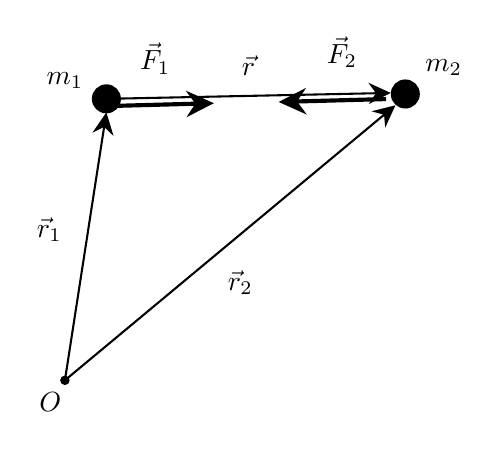
\begin{tikzpicture}[x=0.75pt,y=0.75pt,yscale=-1,xscale=1]
	%uncomment if require: \path (0,300); %set diagram left start at 0, and has height of 300

	%Straight Lines [id:da6863459773640985] 
	\draw    (114.5,238) -- (271.44,107.42) ;
	\draw [shift={(273.75,105.5)}, rotate = 500.24] [fill={rgb, 255:red, 0; green, 0; blue, 0 }  ][line width=0.08]  [draw opacity=0] (10.72,-5.15) -- (0,0) -- (10.72,5.15) -- (7.12,0) -- cycle    ;
	%Straight Lines [id:da5313627472873643] 
	\draw    (114.5,238) -- (134.02,111.87) ;
	\draw [shift={(134.48,108.9)}, rotate = 458.8] [fill={rgb, 255:red, 0; green, 0; blue, 0 }  ][line width=0.08]  [draw opacity=0] (10.72,-5.15) -- (0,0) -- (10.72,5.15) -- (7.12,0) -- cycle    ;
	%Straight Lines [id:da4027192773772521] 
	\draw    (134.48,102.4) -- (268.5,99.61) ;
	\draw [shift={(271.5,99.55)}, rotate = 538.81] [fill={rgb, 255:red, 0; green, 0; blue, 0 }  ][line width=0.08]  [draw opacity=0] (10.72,-5.15) -- (0,0) -- (10.72,5.15) -- (7.12,0) -- cycle    ;
	%Shape: Circle [id:dp5223940100275606] 
	\draw  [fill={rgb, 255:red, 0; green, 0; blue, 0 }  ,fill opacity=1 ] (112.75,238) .. controls (112.75,237.03) and (113.53,236.25) .. (114.5,236.25) .. controls (115.47,236.25) and (116.25,237.03) .. (116.25,238) .. controls (116.25,238.97) and (115.47,239.75) .. (114.5,239.75) .. controls (113.53,239.75) and (112.75,238.97) .. (112.75,238) -- cycle ;
	%Shape: Circle [id:dp597764102802874] 
	\draw  [fill={rgb, 255:red, 0; green, 0; blue, 0 }  ,fill opacity=1 ] (127.98,102.4) .. controls (127.98,98.81) and (130.89,95.9) .. (134.48,95.9) .. controls (138.07,95.9) and (140.98,98.81) .. (140.98,102.4) .. controls (140.98,105.99) and (138.07,108.9) .. (134.48,108.9) .. controls (130.89,108.9) and (127.98,105.99) .. (127.98,102.4) -- cycle ;
	%Shape: Circle [id:dp7278212874749974] 
	\draw  [fill={rgb, 255:red, 0; green, 0; blue, 0 }  ,fill opacity=1 ] (272,100.05) .. controls (272,96.46) and (274.91,93.55) .. (278.5,93.55) .. controls (282.09,93.55) and (285,96.46) .. (285,100.05) .. controls (285,103.64) and (282.09,106.55) .. (278.5,106.55) .. controls (274.91,106.55) and (272,103.64) .. (272,100.05) -- cycle ;
	%Straight Lines [id:da2625538502562448] 
	\draw [line width=1.5]    (134.48,105.9) -- (182.25,104.61) ;
	\draw [shift={(186.25,104.5)}, rotate = 538.45] [fill={rgb, 255:red, 0; green, 0; blue, 0 }  ][line width=0.08]  [draw opacity=0] (13.4,-6.43) -- (0,0) -- (13.4,6.44) -- (8.9,0) -- cycle    ;
	%Straight Lines [id:da010873890958111199] 
	\draw [line width=1.5]    (221.48,103.79) -- (269.25,102.5) ;
	\draw [shift={(217.48,103.9)}, rotate = 358.45] [fill={rgb, 255:red, 0; green, 0; blue, 0 }  ][line width=0.08]  [draw opacity=0] (13.4,-6.43) -- (0,0) -- (13.4,6.44) -- (8.9,0) -- cycle    ;

	% Text Node
	\draw (107.5,248.5) node    {$O$};
	% Text Node
	\draw (107,165.5) node    {$\vec{r}_{1}$};
	% Text Node
	\draw (199,191) node    {$\vec{r}_{2}$};
	% Text Node
	\draw (114.5,93.5) node    {$m_{1}$};
	% Text Node
	\draw (297,87.5) node    {$m_{2}$};
	% Text Node
	\draw (203,86.5) node    {$\vec{r}$};
	% Text Node
	\draw (248,80) node    {$\vec{F}_{2}$};
	% Text Node
	\draw (158,83) node    {$\vec{F}_{1}$};

	\end{tikzpicture}
\end{figure}
\FloatBarrier
Si nota che il vettore $\vec{r}$ che dà la distanza fra i due pianeti, è tale per cui, per costruzione geometrica:

\[
	\vec{r}_1+\vec{r}=\vec{r}_2 \implies \vec{r}=\vec{r}_2-\vec{r}_1
\]

Per studiare un problema di questo tipo si applica il secondo principio della dinamica:

\begin{align*}
	\vec{F}_1 &= m_1\vec{a}_1=m_1\frac{d^2\vec{r}_1}{dt^2} \\
	\vec{F}_2 &= m_1\vec{a}_2=m_2\frac{d^2\vec{r}_2}{dt^2}
\end{align*}

Si dividono le due relazioni membro a membro:

\[
	\frac{\vec{F}_1}{m_1}=\frac{d^2\vec{r}_1}{dt^2} \quad \frac{\vec{F}_2}{m_2}=\frac{d^2\vec{r}_2}{dt^2}
\]

Si sa per il principio di azione reazione che queste due forze $\vec{F}_1$ e $\vec{F}_2$ non sono indipendenti fra di loro ma sono una l'opposta dell'altra. Si chiami allora $\vec{F}$ la forza $\vec{F}_2$, $\vec{F}_1$ sarà semplicemente $-\vec{F}$.

\[
	\vec{F}_2=\vec{F} \quad \vec{F}_1=-\vec{F}
\]

Sottraendo membro a membro:

\[
	\frac{\vec{F}}{m_2}+\frac{\vec{F}}{m_1}=\frac{d^2(\vec{r}_2-\vec{r_1})}{dt^2}
\]

La derivazione è un operazione lineare, quindi fare la differenza delle derivate è uguale a fare la derivata della differenza. Quindi si avrà:

\[
	\vec{F} \biggl(\frac{1}{m_1}+\frac{1}{m_2} \biggr)=\frac{d^2\vec{r}}{dt^2}
\]

A questo punto si può definire una quantità detta \textbf{massa ridotta}, $\mu$, che ha dimensione di una massa ed è tale per cui:

\[
	\frac{1}{\mu}=\biggl(\frac{1}{m_1}+\frac{1}{m_2} \biggr) \implies \vec{F}\frac{1}{\mu}=\frac{d^2\vec{r}}{dt^2} \implies \vec{F}=\mu \frac{d^2\vec{r}}{dt^2}
\]

Si ottiene finalmente una relazione affermante che la forza che genera uno dei due corpi, è uguale alla massa ridotta per la derivata seconda di $\vec{r}$ rispetto al tempo. Quindi, se si vuole studiare il moto di due corpi soggetti entrambi alla mutua interazione gravitazionale, invece che concentrarsi sul moto assoluto di $m_1$ e $m_2$, si può osservare il moto relativo dei due corpi uno rispetto all'altro, semplicemente sostituendo alla massa di uno dei due corpi, la massa ridotta. Si è infatti riscritto il moto in funzione della variabile $\vec{r}$.  Si semplifica il problema dei due corpi nel problema di un corpo solo. Nel caso del moto della Terra intorno al Sole, dove quindi uno dei due corpi è molto molto maggiore in massa dell'altro, si ha:

\[
	M \gg m \implies \frac{1}{\mu}=\frac{1}{M}+\frac{1}{m}  \approx \frac{1}{M} \implies \mu \approx M
\]

Si è immaginato il Sole come fermo, perché fondamentalmente la sua massa è molto maggiore e la massa ridotta diventa semplicemente la massa del pianeta. Se le masse dei due pianeti invece sono di valore simile, allora si deve semplicemente sostituire alla massa di un pianeta, la massa ridotta.

Affrontare il problema dei tre corpi è un problema molto complesso che non ha soluzione analitica. In generale, studiare il moto relativo di un certo numero di corpi soggetti a mutua interazione è molto complicato.
